\chapter{Chemische stoffen, natuurlijk en synthetisch}\label{ch:g10:chemical-species}

Een lepel vanille-ijs. De smaak kan komen van de zwarte peulen van een
tropische orchidee, geplukt, gefermenteerd en maandenlang in alcohol
geweekt; of hij kan komen uit een fabriek die het aroma maakt uit
houtpulp of uit aardolie. Proef ze naast elkaar en de hoofdsmaak is
dezelfde --- met een goede reden: het \omterm{def:g7:atoms-and-molecules:molecule}{molecuul} dat naar vanille smaakt,
vanilline, is precies hetzelfde \omterm{def:g7:atoms-and-molecules:molecule}{molecuul}, hoe het ook verkregen is. Dit
hoofdstuk laat zien hoe scheikundigen een stof uit een plant halen, hoe
ze haar maken, en hoe ze controleren dat ze echt hebben wat ze denken te
hebben.

\begin{recall}
Een \omterm{def:g6:pure-substances-and-mixtures:species}{chemische stof} is één bepaalde soort stof; een \omterm{def:g6:pure-substances-and-mixtures:pure-substance}{zuivere stof} bevat één
\omterm{def:g6:pure-substances-and-mixtures:species}{chemische stof} en heeft vaste constanten, zoals haar smelt- en kookpunt
(\cref{ch:g6:pure-substances-and-mixtures}). Vloeistoffen zijn \omterm{def:g6:solutions-and-solubility:miscible}{mengbaar}
of \omterm{def:g6:solutions-and-solubility:miscible}{niet-mengbaar}, en elke \omterm{def:g6:solutions-and-solubility:solute}{opgeloste stof} heeft in elk \omterm{def:g6:solutions-and-solubility:solute}{oplosmiddel} haar
eigen \omterm{def:g6:solutions-and-solubility:solubility}{oplosbaarheid} (\cref{ch:g6:solutions-and-solubility}).
\omterm{def:g7:identifying-substances:chromatography}{Papierchromatografie} scheidt de kleurstoffen van een \omterm{def:g6:pure-substances-and-mixtures:mixture}{mengsel}
(\cref{ch:g7:identifying-substances}).
\end{recall}

\begin{omfigure}
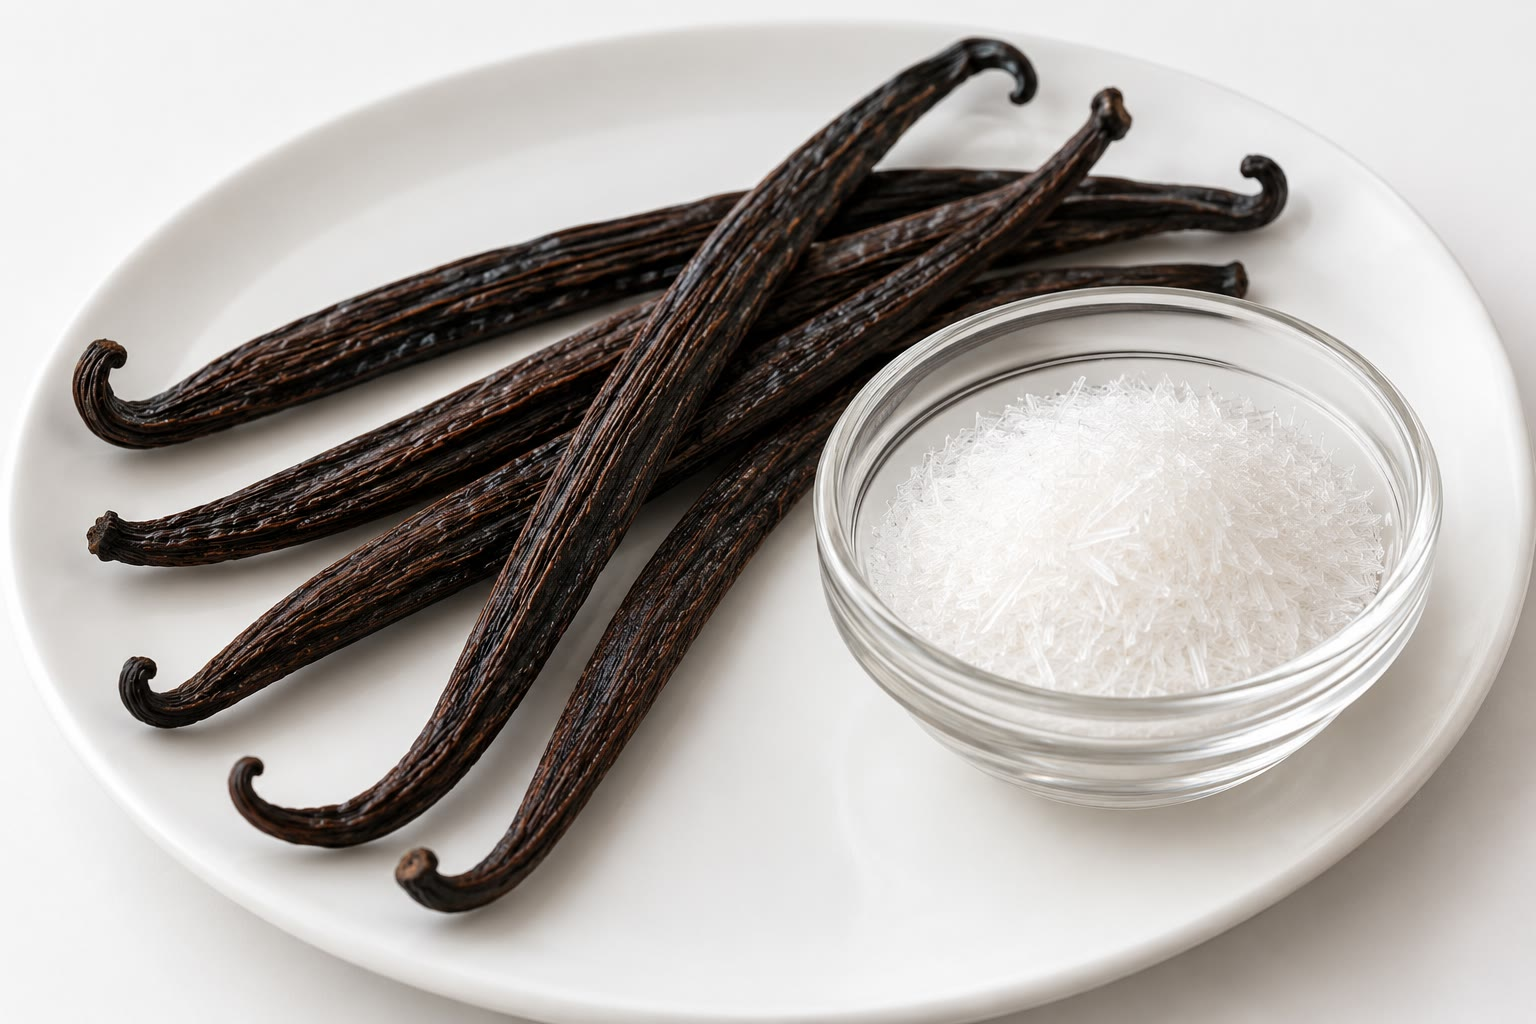
\includegraphics[width=0.55\linewidth]{images/book1/ai/g10-vanilla.jpg}

{\small Vanillestokjes en witte kristallen vanilline: hetzelfde \omterm{def:g7:atoms-and-molecules:molecule}{molecuul},
uit een plant of uit een fabriek.}
\end{omfigure}

\section{Natuurlijke en synthetische stoffen}

\begin{definition}[Natuurlijke en synthetische stoffen]\label{def:g10:chemical-species:natural}
Een \emph{natuurlijke stof}\index{natuurlijke stof} is een \omterm{def:g6:pure-substances-and-mixtures:species}{chemische
stof} die door een levend wezen gemaakt wordt of als zodanig in de natuur
voorkomt. Een \emph{synthetische stof}\index{synthetische stof} wordt
door scheikundigen met \omterm{def:g7:chemical-reactions:reaction}{chemische reacties} uit andere stoffen gemaakt.
Een synthetische stof kan identiek zijn aan een natuurlijke
(synthetische vanilline), of geen tegenhanger in de natuur hebben (de
meeste geneesmiddelen en \omterm{def:g8:plastics:plastic}{kunststoffen}).
\end{definition}

\begin{proposition}[Dezelfde stof, dezelfde eigenschappen]\label{prop:g10:chemical-species:same}
Een \omterm{def:g6:pure-substances-and-mixtures:species}{chemische stof} heeft dezelfde eigenschappen, wat haar herkomst ook
is: vanilline uit een fabriek en vanilline uit een vanillestokje hebben
dezelfde formule, hetzelfde smeltpunt, dezelfde geur. Wat kan
verschillen, is wat er nog bij zit: een natuurlijk extract is een
\omterm{def:g6:pure-substances-and-mixtures:mixture}{mengsel}, met veel andere stoffen die de smaak veranderen.
\end{proposition}

\begin{history}[Van wilgenbast tot aspirine, 1828--1899]
Eeuwenlang werd er op wilgenbast gekauwd tegen koorts en pijn. In 1828
haalde een scheikundige er de werkzame stof uit, salicine; scheikundigen
zetten die daarna om in salicylzuur, dat werkt maar de maag irriteert.
In 1897 maakte Felix Hoffmann bij een fabriek van kleurstoffen en
geneesmiddelen uit salicylzuur een mildere \omterm{def:g10:chemical-species:natural}{synthetische stof}:
acetylsalicylzuur, dat vanaf 1899 als aspirine werd verkocht. Aspirine
heeft geen natuurlijke bron: het is een volledig \omterm{def:g10:chemical-species:natural}{synthetische stof}.
\end{history}

\section{Een stof extraheren}

\begin{definition}[Extractie en vloeistof-vloeistofextractie]\label{def:g10:chemical-species:extraction}
Bij een \emph{extractie}\index{extractie} haal je een \omterm{def:g6:pure-substances-and-mixtures:species}{chemische stof} uit
het materiaal waarin ze zit, meestal door haar op te lossen in een goed
gekozen \omterm{def:g6:solutions-and-solubility:solute}{oplosmiddel}. Bij een
\emph{vloeistof-vloeistofextractie}\index{vloeistof-vloeistofextractie}
gaat een stof die in de ene vloeistof opgelost is over naar een tweede
vloeistof, die niet \omterm{def:g6:solutions-and-solubility:miscible}{mengbaar} is met de eerste en waarin ze beter
\omterm{def:g2:mixing-and-dissolving:dissolve}{oplost}; de twee vloeistoffen worden daarna in een scheitrechter
gescheiden.
\end{definition}

\begin{example}[Extracties in het dagelijks leven]\label{ex:g10:chemical-species:everyday}
Thee zetten is een \omterm{def:g10:chemical-species:extraction}{extractie} met heet water (infusie); vanillestokjes in
alcohol laten weken is een \omterm{def:g10:chemical-species:extraction}{extractie} met ethanol (maceratie); groenten
koken om bouillon te maken is er ook een (decoctie).
\end{example}


\begin{definition}[Destillatie en hydrodestillatie]\label{def:g10:chemical-species:distillation}
Bij een \emph{destillatie}\index{destillatie} verhit je een
vloeistofmengsel tot het kookt, laat je de damp weer vloeibaar worden in
een koeler die met stromend water gekoeld wordt, en vang je die
vloeistof op, het destillaat. Bij een
\emph{hydrodestillatie}\index{hydrodestillatie} kook je plantenmateriaal
in water: de stoom neemt de geurstoffen van de plant mee, die zich in
het destillaat als een olieachtige laag van het water scheiden, de
etherische olie.
\end{definition}

\begin{omfigure}
\begin{tikzpicture}[font=\small, scale=0.95]
  \pic[transform shape] at (0,0) {heatingmantle};
  \pic[transform shape] at (0,0) {rbflask={0.55}{omWater!70}};
  \foreach \x/\y in {-0.45/0.35,-0.1/0.55,0.3/0.3,0.5/0.7,-0.6/0.75,0.1/0.9,-0.25/0.2}
    \fill[green!45!black!70] (\x,\y) ellipse (0.09 and 0.04);
  \pic[transform shape] (s) at (0,3.0) {stillhead};
  \pic[transform shape] at ($(s-top)+(0,-0.75)$) {thermometer};
  \pic[transform shape, rotate=-20] (c) at (s-arm) {liebig={3.2}};
  \coordinate (cend) at ($(s-arm)+(-20:3.2)$);
  \pic[transform shape] (a) at (cend) {adapter};
  \pic[transform shape] at ($(a-tip)+(0,-2.3)$) {erlenmeyer={0.18}{omWater!70}};
  \fill[yellow!60!orange!60] ($(a-tip)+(-0.827,-2.3+0.47)$) -- ($(a-tip)+(0.827,-2.3+0.47)$) -- ($(a-tip)+(0.779,-2.3+0.6)$) -- ($(a-tip)+(-0.779,-2.3+0.6)$) -- cycle;
  \draw[<-, omProp, thick] (-0.55,0.55) -- (-2.2,0.9) node[left, text=black, align=right]
    {water en\\ lavendelbloemen};
  \draw[<-, omProp, thick] (1.35,-0.6) -- (2.2,-1.1) node[right, text=black]
    {verwarmingsmantel};
  \draw[<-, omProp, thick] (0.1,4.2) -- (-1.2,4.6) node[left, text=black] {thermometer};
  \draw[<-, omProp, thick] ($(s-arm)+(-20:1.6)+(0,0.32)$) -- ++(0.6,1.0) node[above, text=black]
    {koeler, gekoeld met stromend water};
  \draw[<-, omProp, thick] ($(a-tip)+(0.4,-1.88)$) -- ++(1.1,0.2) node[right, text=black, align=left]
    {destillaat: etherische olie\\ drijvend op water};
\end{tikzpicture}

{\small \omterm{def:g10:chemical-species:distillation}{Hydrodestillatie} van lavendel. De stoom voert de etherische olie
naar de koeler; het destillaat scheidt zich in een dun laagje olie
bovenop water.}
\end{omfigure}

\begin{method}[Een extractiemiddel kiezen]\label{met:g10:chemical-species:solvent}
Voor een \omterm{def:g10:chemical-species:extraction}{vloeistof-vloeistofextractie} van een stof uit water moet het
\omterm{def:g6:solutions-and-solubility:solute}{oplosmiddel}:
\begin{enumerate}
  \item de stof veel beter \omterm{def:g2:mixing-and-dissolving:dissolve}{oplossen} dan water;
  \item niet \omterm{def:g6:solutions-and-solubility:miscible}{mengbaar} zijn met water, zodat er twee lagen ontstaan;
  \item zo weinig mogelijk gevaarlijk zijn, en achteraf makkelijk te
        verwijderen (een laag kookpunt laat het verdampen).
\end{enumerate}
Welke laag bovenop ligt, bepalen de dichtheden: de minst dichte vloeistof
drijft.
\end{method}

\begin{example}[Oplosmiddelen voor lavendelolie]\label{ex:g10:chemical-species:table}
% ledger: rho:cyclohexane, bp:cyclohexane, rho:ethyl-acetate, bp:ethyl-acetate, rho:CH2Cl2, bp:CH2Cl2, rho:ethanol, bp:ethanol, sol:linalool
Linalool, de belangrijkste stof van lavendelolie, lost maar tot
\qty{1.6}{g/L} op in water, maar heel goed in de \omterm{def:g6:solutions-and-solubility:solute}{oplosmiddelen} hieronder:
\begin{center}
\small
\begin{tabular}{lccll}
\hline
\omterm{def:g6:solutions-and-solubility:solute}{oplosmiddel} & massa van \qty{1}{mL} & kookpunt & met water & voornaamste gevaren \\
\hline
cyclohexaan & \qty{0.78}{g} & \qty{81}{\celsius} & niet \omterm{def:g6:solutions-and-solubility:miscible}{mengbaar} & ontvlambaar, schadelijk \\
ethylethanoaat & \qty{0.90}{g} & \qty{77}{\celsius} & niet \omterm{def:g6:solutions-and-solubility:miscible}{mengbaar} & ontvlambaar, irriterend \\
dichloormethaan & \qty{1.33}{g} & \qty{40}{\celsius} & niet \omterm{def:g6:solutions-and-solubility:miscible}{mengbaar} & verdacht kankerverwekkend \\
ethanol & \qty{0.79}{g} & \qty{78}{\celsius} & \omterm{def:g6:solutions-and-solubility:miscible}{mengbaar} & ontvlambaar \\
\hline
\end{tabular}
\end{center}
Ethanol is onbruikbaar: het \omterm{def:g2:mixing-and-dissolving:mix}{mengt} met water en er ontstaan geen lagen.
Met cyclohexaan of ethylethanoaat ligt de laag van het \omterm{def:g6:solutions-and-solubility:solute}{oplosmiddel}
bovenop; met dichloormethaan onderaan.
\end{example}

\begin{omfigure}
\begin{tikzpicture}[font=\small, scale=1.2]
  \pic[transform shape] at (0,0) {sepfunnel={omWater!70}{yellow!35!orange!35}};
  \draw[<-, omProp, thick] (0.55,2.1) -- (1.6,2.4) node[right, text=black, align=left]
    {cyclohexaan met de olie\\ (minder dicht, bovenop)};
  \draw[<-, omProp, thick] (0.55,1.3) -- (1.6,1.2) node[right, text=black, align=left]
    {water, afgetapt\\ via de kraan};
  \draw[<-, omProp, thick] (0.25,0.52) -- (1.6,0.4) node[right, text=black] {kraan};
\end{tikzpicture}

{\small Een scheitrechter na schudden en laten \omterm{def:g3:separating-mixtures:decant}{bezinken}: de olie is
overgegaan naar het cyclohexaan, bovenop.}
\end{omfigure}

\begin{safety}{\ghs[0.8cm]{GHS02}\ghs[0.8cm]{GHS07}\ghs[0.8cm]{GHS08}\ghs[0.8cm]{GHS09}}
% ledger: ghs:cyclohexane
Cyclohexaan: zeer licht ontvlambaar (GHS02); kan dodelijk zijn als het
wordt ingeslikt en in de luchtwegen terechtkomt, veroorzaakt
huidirritatie en slaperigheid (GHS07, GHS08); zeer giftig voor in het
water levende organismen (GHS09). Gebruik in een zuurkast, ver van
vlammen.
\end{safety}

\section{Dunnelaagchromatografie}

\begin{definition}[Dunnelaagchromatografie]\label{def:g10:chemical-species:tlc}
\emph{Dunnelaagchromatografie}\index{dunnelaagchromatografie} (DLC)
scheidt de stoffen van een \omterm{def:g6:pure-substances-and-mixtures:mixture}{mengsel} op een plaatje dat bedekt is met een
dun laagje fijn wit poeder, de \emph{stationaire fase}\index{stationaire fase}.
Kleine stipjes van de monsters worden op een potloodlijn vlak boven de
onderkant gezet; het plaatje staat in een afgesloten bak in een beetje
\omterm{def:g6:solutions-and-solubility:solute}{oplosmiddel}, het \emph{eluens}\index{eluens}, dat in het plaatje
omhoogkruipt en elke stof meeneemt tot een hoogte die van de stof
afhangt. Kleurloze vlekken maak je daarna zichtbaar onder ultraviolet
licht of met jooddamp.
\end{definition}

\begin{definition}[Retentiefactor]\label{def:g10:chemical-species:retention-factor}
De \emph{retentiefactor}\index{retentiefactor} van een vlek is
\[
  R_f = \frac{\text{afstand van de startlijn tot de vlek}}
             {\text{afstand van de startlijn tot het front van het eluens}},
\]
een getal tussen 0 en 1. Bij een gegeven plaatje, \omterm{def:g10:chemical-species:tlc}{eluens} en temperatuur
heeft elke stof haar eigen $R_f$.
\end{definition}

\begin{method}[Een DLC uitvoeren en aflezen]\label{met:g10:chemical-species:tlc}
\begin{enumerate}
  \item Trek de startlijn met potlood, \qty{1}{cm} van de onderkant; zet
        er een klein stipje op van elk monster en van elke
        referentiestof.
  \item Zet het plaatje in de bak, het \omterm{def:g10:chemical-species:tlc}{eluens} onder de lijn; sluit de
        bak.
  \item Haal het plaatje eruit als het front ongeveer \qty{1}{cm} onder
        de bovenkant is; markeer het front meteen; laat drogen en maak
        zichtbaar.
  \item Meet de afstanden en bereken de $R_f$ van elke vlek. Een monster
        dat één vlek geeft, is waarschijnlijk een \omterm{def:g6:pure-substances-and-mixtures:pure-substance}{zuivere stof}; een vlek
        op dezelfde hoogte als een referentievlek op hetzelfde plaatje is
        waarschijnlijk die stof.
\end{enumerate}
\end{method}

\begin{omfigure}
\begin{tikzpicture}[font=\small, scale=1.25]
  % the tank
  \pic[transform shape] at (0,0) {beaker={0.15}{omWater!80}};
  \fill[white] (-0.55,0.08) rectangle (0.55,1.92);
  \fill[omWater!80] (-0.55,0.08) rectangle (0.55,0.3);
  \draw[omGlass, line width=0.6pt] (-0.55,0.08) rectangle (0.55,1.92);
  \draw[black!60] (-0.55,0.42) -- (0.55,0.42);
  \foreach \x in {-0.3,0,0.3} \fill[black!70] (\x,0.42) circle (0.04);
  \fill[black!25] (-1.0,2.08) rectangle (1.0,2.18);
  \node[anchor=north, align=center] at (0,-0.15) {de bak, gesloten\\ met een deksel};
  % the developed plate
  \begin{scope}[xshift=4.2cm]
    \pic[transform shape] at (0,0) {tlcplate};
    \draw[black!50, dashed] (-0.7,2.8) -- (0.7,2.8);
    \fill[omDef!70] (-0.35,1.36) ellipse (0.1 and 0.07);
    \fill[omDef!70] (-0.35,2.2) ellipse (0.1 and 0.07);
    \fill[omDef!70] (0,1.36) ellipse (0.1 and 0.07);
    \fill[omDef!70] (0.35,2.2) ellipse (0.1 and 0.07);
    \foreach \x/\l in {-0.35/O,0/L,0.35/A} \node[font=\footnotesize, anchor=north] at (\x,0.38) {\l};
    \draw[<->, omProp] (0.95,0.4) -- (0.95,1.36) node[midway, right, text=black, font=\footnotesize] {$d$};
    \draw[<->, omProp] (1.55,0.4) -- (1.55,2.8) node[midway, right, text=black, font=\footnotesize] {$D$};
    \draw[black!40, densely dotted] (-0.25,1.36) -- (0.95,1.36);
    \node[anchor=north, align=center] at (0.2,-0.15) {het ontwikkelde plaatje:\\ $R_f = d/D$};
  \end{scope}
\end{tikzpicture}

{\small DLC van lavendelolie (O) naast linalool (L) en linalylethanoaat
(A). De olie geeft twee vlekken, op de hoogte van de twee referenties:
ze bevat beide stoffen. Voor linalool geldt $R_f = d/D$.}
\end{omfigure}

\section{Een stof herkennen aan haar fysische constanten}

\begin{proposition}[Een smeltpunt controleert identiteit en zuiverheid]\label{prop:g10:chemical-species:mp}
% ledger: mp:vanillin, mp:aspirin, mp:salicylic
Een zuivere vaste stof smelt scherp bij haar eigen temperatuur:
vanilline bij ongeveer \qty{82}{\celsius}, aspirine bij
\qty{135}{\celsius}, salicylzuur bij \qty{158}{\celsius}. Een onzuiver
monster smelt lager, en over een traject van enkele graden. Een
smeltpunt meten, op een verwarmde \omterm{def:g9:periodic-table-first-look:metal}{metalen} bank (Koflerbank) of in een
smeltpuntapparaat, laat dus zowel zien welke vaste stof het is als of
ze zuiver is.
\end{proposition}

\begin{inthelab}[Een DLC-plaatje]
De leerlingen stippen lavendelolie, linalool en linalylethanoaat op een
plaatje, ontwikkelen het in een afgesloten pot met een \omterm{def:g6:pure-substances-and-mixtures:mixture}{mengsel} van
\omterm{def:g6:solutions-and-solubility:solute}{oplosmiddelen} dat de docent heeft gekozen, en maken het zichtbaar onder
een uv-lamp, met een bril die het ultraviolet tegenhoudt. Het \omterm{def:g10:chemical-species:tlc}{eluens}
wordt in de zuurkast gebruikt en gehanteerd.
\end{inthelab}

\begin{omfigure}
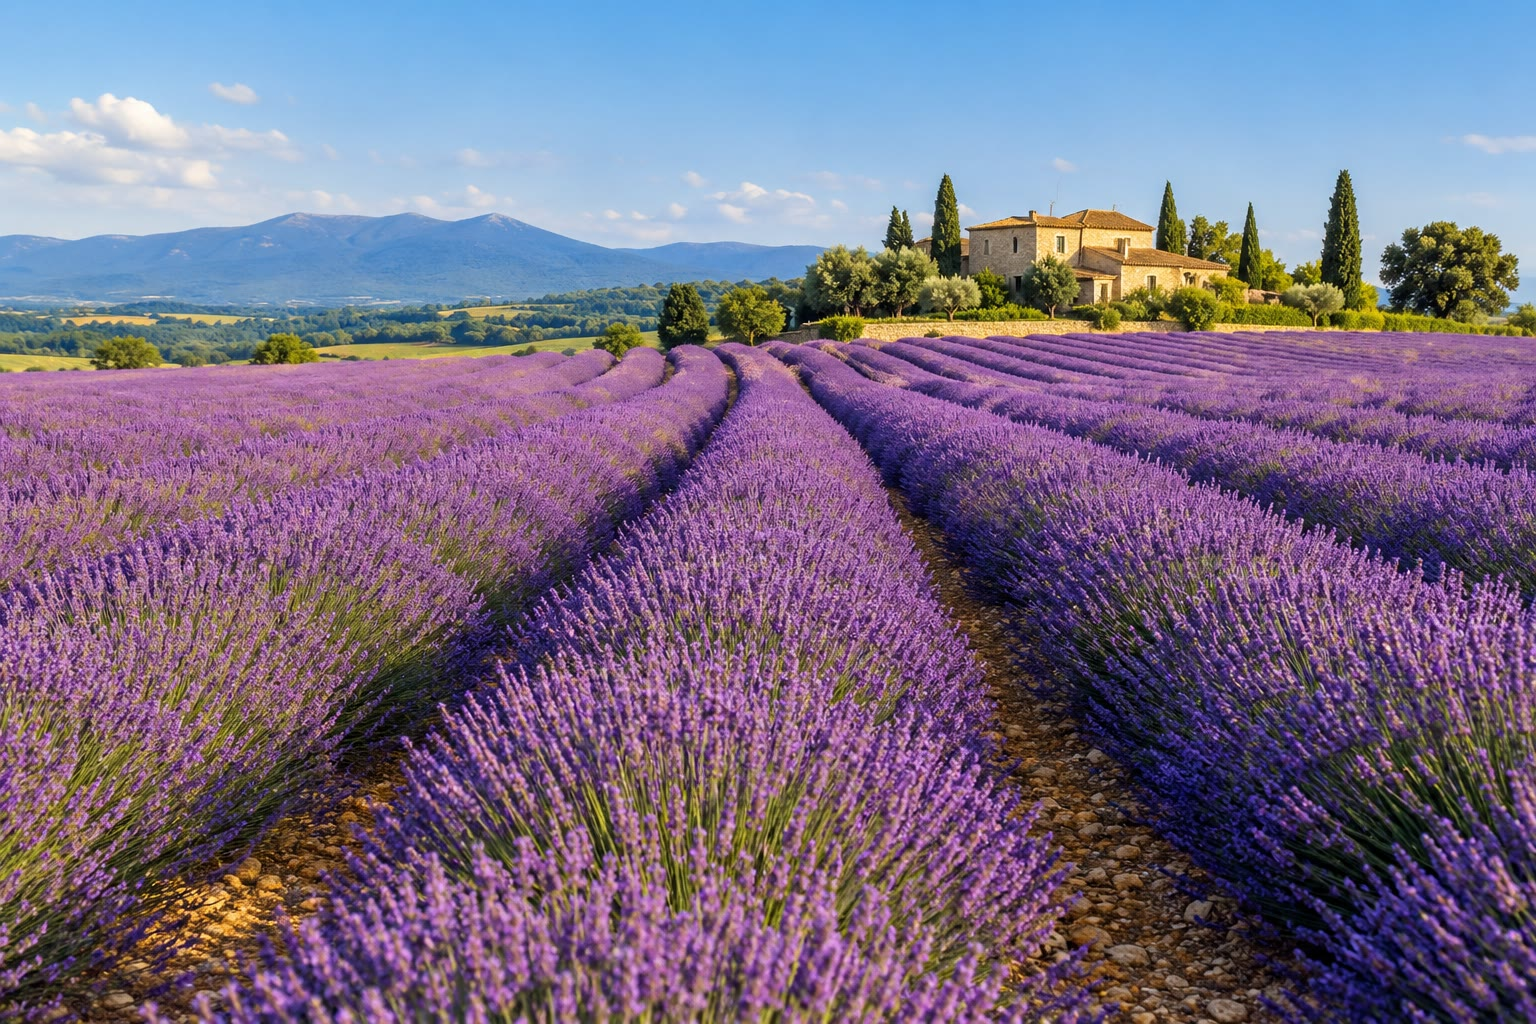
\includegraphics[width=0.55\linewidth]{images/book1/ai/g10-lavender-field.jpg}

{\small Een bloeiend lavendelveld: de \omterm{def:g5:raw-materials-and-recycling:raw-material}{grondstof} van etherische
lavendelolie.}
\end{omfigure}

\section{Oefeningen}

\begin{exercise}[$\star$]\label{exo:g10:chemical-species:1}
Natuurlijke of \omterm{def:g10:chemical-species:natural}{synthetische stof}? Vanilline uit een vanillestokje;
aspirine; cafeïne uit koffiebonen; vanilline uit een fabriek.
\end{exercise}

\begin{exercise}[$\star$]\label{exo:g10:chemical-species:2}
Waarom hebben synthetische en natuurlijke vanilline hetzelfde smeltpunt?
\end{exercise}

\begin{exercise}[$\star$]\label{exo:g10:chemical-species:3}
Op een DLC-plaatje ligt het front van het \omterm{def:g10:chemical-species:tlc}{eluens} \qty{6.0}{cm} boven de
startlijn en een vlek \qty{2.4}{cm} erboven. Bereken haar $R_f$.
\end{exercise}

\begin{exercise}[$\star$]\label{exo:g10:chemical-species:4}
Geef de rol van de koeler bij een \omterm{def:g10:chemical-species:distillation}{destillatie}, en zeg waarom het koude
water aan de onderkant binnenkomt.
\end{exercise}

\begin{exercise}[$\star$]\label{exo:g10:chemical-species:5}
Noem de drie voorwaarden waaraan een extractiemiddel moet voldoen.
\end{exercise}

\begin{exercise}[$\star\star$]\label{exo:g10:chemical-species:6}
Leg met de tabel van \omterm{def:g6:solutions-and-solubility:solute}{oplosmiddelen} uit waarom je linalool niet met
ethanol uit het destillaat kunt extraheren, en wel met cyclohexaan.
\end{exercise}

\begin{exercise}[$\star\star$]\label{exo:g10:chemical-species:7}
In een scheitrechter wordt dichloormethaan met water geschud. Welke laag
ligt bovenop? Verklaar met de tabel.
\end{exercise}

\begin{exercise}[$\star\star$]\label{exo:g10:chemical-species:8}
Een wit poeder dat als aspirine verkocht wordt, begint te smelten bij
\qty{126}{\celsius} en is helemaal gesmolten bij \qty{132}{\celsius}.
Wat kun je concluderen?
\end{exercise}

\begin{exercise}[$\star\star$]\label{exo:g10:chemical-species:9}
Kijk naar de DLC-figuur van dit hoofdstuk. Wat bevat de lavendelolie?
Welke stof is het hoogst gekomen?
\end{exercise}

\begin{exercise}[$\star\star$]\label{exo:g10:chemical-species:10}
Zet de stappen om in het laboratorium lavendelolie te verkrijgen in de
goede volgorde: de lagen scheiden; \omterm{def:g10:chemical-species:distillation}{hydrodestillatie}; cyclohexaan aan het
destillaat toevoegen en schudden; het cyclohexaan laten verdampen.
\end{exercise}

\begin{exercise}[$\star\star$]\label{exo:g10:chemical-species:11}
Waarom trek je de startlijn van een DLC-plaatje met potlood, en waarom
ligt ze boven het \omterm{def:g10:chemical-species:tlc}{eluens}?
\end{exercise}

\begin{exercise}[$\star\star\star$]\label{exo:g10:chemical-species:12}
Na de \omterm{def:g10:chemical-species:extraction}{extractie} wordt het cyclohexaan verwijderd door zacht verwarmen,
zodat de olie achterblijft. Leg met de kookpunten van cyclohexaan en van
linalool (\qty{198}{\celsius}) uit waarom dat werkt.
\end{exercise}

\begin{exercise}[$\star\star\star$]\label{exo:g10:chemical-species:13}
Een synthetisch monster van een aroma geeft één vlek op een
DLC-plaatje, op de hoogte van de \omterm{def:g10:chemical-species:natural}{natuurlijke stof}, en smelt scherp bij
de juiste temperatuur. Welke twee conclusies kun je trekken?
\end{exercise}

\begin{exercise}[$\star\star\star$]\label{exo:g10:chemical-species:14}
Op hetzelfde DLC-plaatje heeft vlek A $R_f = 0.40$ en ligt het front
\qty{5.5}{cm} boven de lijn. Op welke hoogte ligt vlek A? Een andere stof
heeft $R_f = 0.75$: hoe ver boven vlek A ligt ze?
\end{exercise}

\begin{exercise}[$\star\star\star$]\label{exo:g10:chemical-species:15}
In \qty{1}{L} water kan \qty{1.6}{g} linalool \omterm{def:g2:mixing-and-dissolving:dissolve}{oplossen}. Een destillaat
van \qty{200}{mL} water bevat \qty{0.20}{g} opgelost linalool. Is het
verzadigd? Hoeveel zou er nog in kunnen \omterm{def:g2:mixing-and-dissolving:dissolve}{oplossen}? Waarom is het de moeite
waard dit water met cyclohexaan te extraheren in plaats van het weg te
gooien?
\end{exercise}

\clearpage % houdt de kop bij het kader van het probleem (hij bleef onderaan een pagina achter)
\section{Probleem: De geur van lavendel}

\begin{problem}[{Weekendprobleem --- van een mand lavendelbloemen tot een
paar druppels etherische olie, gecontroleerd met chromatografie}]
\label{pb:g10:chemical-species:1}
% ledger: rho:cyclohexane, bp:cyclohexane, rho:CH2Cl2, bp:linalool, ghs:cyclohexane
In een schoollaboratorium wordt \qty{100}{g} verse lavendelbloemen met
water gehydrodestilleerd. Het destillaat, troebel, wordt in een
scheitrechter geschud met \qty{20}{mL} cyclohexaan; de cyclohexaanlaag
wordt bewaard en gedroogd, en het cyclohexaan wordt door zacht verwarmen
verdampt. Wat overblijft, is etherische lavendelolie. Gebruik de tabel
van \omterm{def:g6:solutions-and-solubility:solute}{oplosmiddelen} van dit hoofdstuk.

\medskip
\noindent\textbf{Deel I --- De \omterm{def:g10:chemical-species:distillation}{hydrodestillatie}.}
\begin{enumerate}
  \item Wat is de rol van het kokende water bij een \omterm{def:g10:chemical-species:distillation}{hydrodestillatie}?
  \item Wat is de rol van de koeler? Waar komt het koude water erin?
  \item Het destillaat vertoont een dun olieachtig laagje dat op water
        drijft. Is de olie \omterm{def:g6:solutions-and-solubility:miscible}{mengbaar} met water? Is ze meer of minder dicht
        dan water?
  \item Waarom giet je het destillaat niet gewoon af om de olie terug te
        krijgen?
\end{enumerate}

\medskip
\noindent\textbf{Deel II --- De \omterm{def:g10:chemical-species:extraction}{extractie}.}
\begin{enumerate}[resume]
  \item Waarom is cyclohexaan een geschikt \omterm{def:g6:solutions-and-solubility:solute}{oplosmiddel} voor deze
        \omterm{def:g10:chemical-species:extraction}{extractie}?
  \item Zou je in plaats daarvan ethanol kunnen gebruiken? Leg uit.
  \item Ligt de cyclohexaanlaag na schudden en \omterm{def:g3:separating-mixtures:decant}{bezinken} bovenop of
        onderaan? Hoe zou dat zijn met dichloormethaan?
  \item Geef twee voorzorgsmaatregelen die de pictogrammen van
        cyclohexaan vereisen.
  \item Waarom kun je het cyclohexaan laten verdampen zonder het linalool,
        dat kookt bij \qty{198}{\celsius}, te verliezen?
\end{enumerate}

\medskip
\noindent\textbf{Deel III --- De chromatografie.}
De olie, zuiver linalool (L) en zuiver linalylethanoaat (A) worden op een
DLC-plaatje gestipt. Na het ontwikkelen ligt het front \qty{6.0}{cm}
boven de startlijn. De olie geeft twee vlekken, op \qty{2.4}{cm} en
\qty{4.5}{cm}; vlek L ligt op \qty{2.4}{cm}, vlek A op \qty{4.5}{cm}.
\begin{enumerate}[resume]
  \item Bereken de $R_f$ van linalool en van linalylethanoaat.
  \item Wat bevat de olie, voor zover dit plaatje laat zien?
  \item Is lavendelolie een \omterm{def:g6:pure-substances-and-mixtures:pure-substance}{zuivere stof}?
  \item Waarom zijn de referenties op hetzelfde plaatje gestipt als de
        olie?
  \item Synthetisch linalool wordt gestipt op een ander plaatje,
        ontwikkeld onder dezelfde omstandigheden: de vlek heeft
        $R_f = 0.40$. Wat kun je concluderen?
\end{enumerate}

\medskip
\noindent\textbf{Deel IV --- Hoeveel olie?}
De verkregen olie vult \qty{1.0}{mL}; \qty{1}{mL} van deze olie weegt
\qty{0.90}{g}.
\begin{enumerate}[resume]
  \item Hoeveel olie is er verkregen?
  \item Welk percentage van de massa van de bloemen is dat?
  \item Hoeveel bloemen zijn er nodig voor \qty{100}{g} olie?
  \item De olie heet ``natuurlijk''. In welke zin klopt dat? Is haar
        linalool anders dan synthetisch linalool?
  \item Geef de massa etherische olie die uit \qty{100}{g} bloemen
        verkregen wordt.
\end{enumerate}
\end{problem}
